% Modelo de relatório no estilo artigo em duas colunas
\documentclass[twocolumn]{article}
\usepackage[utf8]{inputenc}
\usepackage{amsmath}
\usepackage{subcaption}
\usepackage{mathtools}
\usepackage{graphicx}
\usepackage{color}
\usepackage{authblk}
\usepackage{lmodern}
% \usepackage[colorlinks,citecolor=black,urlcolor=black,bookmarks=false,hypertexnames=true]{hyperref}
\usepackage{geometry}
\usepackage{pdfpages}
\usepackage{fancyhdr}
\usepackage[utf8]{inputenc}

\usepackage[sorting=none,style=numeric]{biblatex}
\addbibresource{refs.bib}
\usepackage[justification=centering]{caption}
\usepackage{makecell}
\usepackage{booktabs}
\usepackage{hhline}
\usepackage{amsmath}
\usepackage{amssymb}
\usepackage{soul}
\usepackage{gensymb}
\usepackage{listings}

\setlength\parindent{0pt}


\newcommand{\myname}{Nishant Aswani}
\newcommand{\mynetid}{nsa325}
\newcommand{\myemail}{nsa325@nyu.edu}
\newcommand{\myhwtype}{Lab }
\newcommand{\myhwnum}{4}
\newcommand{\mycoursenumber}{ENGR-UH 3511}
\newcommand{\myclassname}{Computer Organization and Architecture}
\newcommand{\myassignmenttitle}{Microprocessor Design and Verilog HDL: Part 2}
\newcommand{\myinstructor}{Cristoforos Vasilatos}

\newcommand{\cc}[1]{\texttt{#1}}

\lstset{
  basicstyle=\ttfamily,
  escapeinside=||
}

% Tamanho das margens:
% \geometry{
% 	a4paper,
% 	total={170mm,257mm},
% 	left=30mm,
% 	top=20mm,
% }
%%%%%%%%%%%%%%%%%%%%%%%%%%%%%%%%%%%%%%%%%
% Bibliografia estilo ABNT. Se não tiver instalado, comente a linha abaixo.
% \usepackage[alf, abnt-etal-list=0, abnt-emphasize=bf,abnt-last-names=bibtex, abnt-etal-text=it, abnt-etal-cite=2]{abntex2cite}
%%%%%%%%%%%%%%%%%%%%%%%%%%%%%%%%%%%%%%%%%

% Dados de identificação
\title{\myassignmenttitle}
\author{\myname, \myemail}
\affil{\myclassname (\mycoursenumber), Instructor \myinstructor}
\date{}

\begin{document}
%%%%%%%%%%%%%%%%%%%%%%%%%%%%%%%%%%%%%%%%%%%%%%%% COVER PAGE %%%%%%%%%%%%%%%%%%%%%%%%%%%%%%%%%%%%%%%%%%%%%%%%%%%%
\onecolumn
\pagestyle{fancy}
\fancyhf{}
\renewcommand{\headrulewidth}{0pt}
\rhead{\textbf{Division of Engineering}}
\lhead{\textbf{NYU Abu Dhabi}}

\begin{center}
  
\includegraphics[scale=0.15]{etc/NYUAD-alt-logo.jpg}
\end{center}

{\vspace{2.5em}}

\begin{center}
    \Huge{\textbf{\mycoursenumber}}\\
    {\vspace{0.5em}}
    \Huge{\textbf{\myclassname}}
\end{center}

{\vspace{10em}}

\begin{center}
  \begin{tabular}{|rp{5.0cm}lll|}
    \hline
    &  &  &  & \\
    &  &  &  & \\
    \Large{\textbf{Name:}} & \Large{\myname}
    
    \  &  &  & \\
    \Large{\textbf{Net ID:}} & \Large{\mynetid}
    
    \  &  &  & \\
    \Large{\textbf{Assignment Title:}} & \Large{\myhwtype \myhwnum}
    
    \
    
    \  &  &  & \\
    \hline
  \end{tabular}
\end{center}

\

{\newpage}
%%%%%%%%%%%%%%%%%%%%%%%%%%%%%%%%%%%%%%%%%%%%%%%% COVER PAGE %%%%%%%%%%%%%%%%%%%%%%%%%%%%%%%%%%%%%%%%%%%%%%%%%%%%

\maketitle        

% Resumo de no máximo 200 palavras
% \begin{abstract}
% Este documento orienta a descrição das atividades práticas desenvolvidas em laboratório. São usados como exemplo conceitos da Aula 01 de Acionamentos Elétricos sobre partida direta de motor de indução trifásico. Nesta atividade, um motor é acionado com conexões estrela e triângulo a vazio. As correntes nominais e de partida são medidas com amperímetro analógico e comparadas entre si. Nota-se que, mesmo sem carga, as corrente em estrela são maiores. 
% \end{abstract}

\section{Introduction}

The MIPs CPU operates on the interconnection between several components. However, connecting these components is not as trivial as wiring them together. Often, because of the varied nature of the instructions, certain signals must be selected over others as inputs for a components. Hence, the CPU uses multiplexers (MUX) as well as control logic to select on these multiplexers. \\

The following lab uses Verilog to continue an implementation of a 32-bit MIPS CPU. The modules implemented include a program counter, instruction memory, register file, ALU, data memory, multiple MUXes, half-adders, sign-extension, and control logic

\section{Methodology}

A top-level module was generated through which the several CPU modules were connected. Output from a given module was connected to a wire in the top-level module. This wire was then used as an input for another module. \\

A testbench for the top-level moodule was used to test the CPU; the testbench was able to show  the signals from all of the modules below. 

\section{Results}

\subsection{Assembly Program 1}

The first assembly program consists of the following instructions

\begin{lstlisting}
    mem[0] <= 32'h00000000;    // EMPTY
    mem[1] <= 32'h21290001;    //ADDI $t1 $t1 1
    mem[2] <= 32'h214A0002;    //ADDI $t2 $t2 2
    mem[3] <= 32'h21290001;    //ADDI $t1 $t1 1
    mem[4] <= 32'h214A0002;    //ADDI $t2 $t2 2
\end{lstlisting}

The screenshot below shows the clocked program counter (PC) and instruction memory (IM). We see that there is a one cycle delay between each of the outputs. This is because the PC and IM are clocked.


\begingroup
    \centering
    \medskip
    %width=\columnwidth
    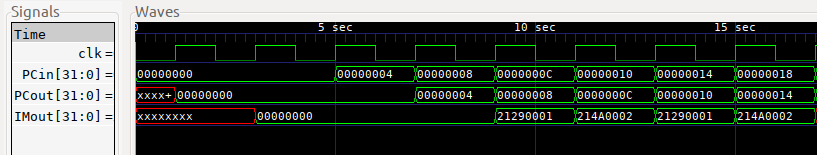
\includegraphics[width=\columnwidth]{Lab-Tex/Lab4-images/p1_1.png}
    \captionof{figure}{Wave output of program counter and instruction memory output}
    \medskip
\endgroup

The instruction output is sliced, and there is a decision to be made for what must be fed into the register file. Hence, we have a mux that selects between \cc{IMout[20:16]} and \cc{IMout[15:11]} for the write register address. Below, we see that the mux selects for \cc{IMout[20:16]} because that slice contains the target registers, such as \cc{\$t1} and \cc{\$t2}.

\begingroup
    \centering
    \medskip
    %width=\columnwidth
    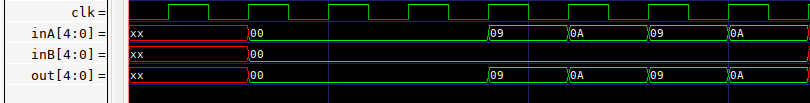
\includegraphics[width=\columnwidth]{Lab-Tex/Lab4-images/p1_2.png}
    \captionof{figure}{Wave output instruction memory mux}
    \medskip
\endgroup

In parallel, the CPU must sign extend the 16 bits of the immediate value to 32 bits to be used in the ALU. \\
\vspace{0.5em}
\begingroup
    \centering
    \medskip
    %width=\columnwidth
    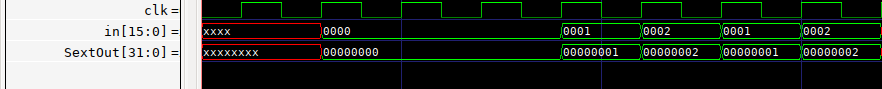
\includegraphics[width=\columnwidth]{Lab-Tex/Lab4-images/p1_3.png}
    \captionof{figure}{Wave output instruction memory mux}
    \medskip
\endgroup
Finally, we send the sign extended immediate value and the output of readRegisterOne (which is readDataOne) into the ALU and we receive an output that is the sum of the two inputs.\\
\vspace{0.5em}
\begingroup
    \centering
    \medskip
    %width=\columnwidth
    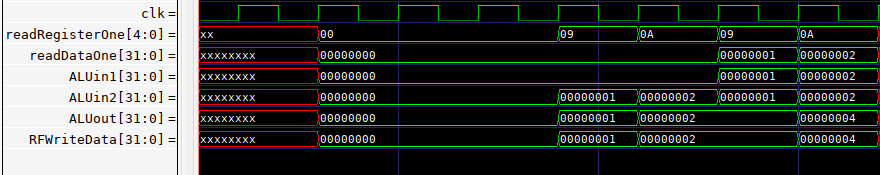
\includegraphics[width=\columnwidth]{Lab-Tex/Lab4-images/p1_4.png}
    \captionof{figure}{Wave output ALU}
    \medskip
\endgroup

\newpage

Notice that the \cc{readDataOne} and \cc{ALUin1} signals are identical. Also notice that the \cc{ALUout} and \cc{writeData} signals are identical. The latter is because the mux handling register writing selects the ALU output in this case, since it is not a load word instruction.\\

As expected, the writeData signal outputs: 1, 2, 2, and 4. Both registers \cc{\$t1} and \cc{\$t2} initially hold 0s. 1 is added to \cc{\$t1} twice and 2 is added to \cc{\$t2} twice. The output wave shows the values in the registers. testReg1 refers to \cc{\$t1} and testReg2 refers to \cc{\$t2}.\\

\begingroup
    \centering
    \medskip
    %width=\columnwidth
    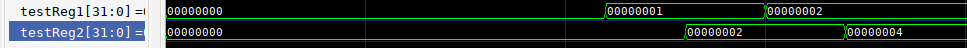
\includegraphics[width=\columnwidth]{Lab-Tex/Lab4-images/p1_5.png}
    \captionof{figure}{Wave output ALU}
    \medskip
\endgroup

Thus, this program demonstrates the CPU's ability to fetch instructions from memory, read/write from a register, and compute something in the ALU.

\subsection{Assembly Program 2}

The second assembly program is as follows

\begin{lstlisting}
    mem[0] <= 32'h00000000;    // EMPTY
    mem[1] <= 32'hAD2A0000;    //SW $t2 0($t1)
    mem[2] <= 32'h8D290000;    //LW $t1 0($t1)
\end{lstlisting}
\\
Because the data memory control signals vary between the two instructions, some additional control logic was added to the top-level module:\\

\begin{lstlisting}
  always@(*) begin
    // store word
    if(IMout[31:26] == 6'b101011) begin
      memWrite <= 1;
      memRead <= 0;
      RegWrite = 0;
    end

    // load word
    else if (IMout[31:26] == 6'b100011) begin
      memWrite <= 0;
      memRead <= 1;
      RegWrite = 1;
    end

    else begin
      memWrite <= 0;
      memRead <= 0;
    end
  end
\end{lstlisting}

\newpage

The logic above ensures that the \cc{memRead, memWrite, and regWrite} signals function are as needed for the \cc{sw} and \cc{lw} instructions.\\

Once again, the screenshot below shows the clocked program counter (PC) and instruction memory (IM). We see that there is a one cycle delay between each of the outputs because the PC and IM are clocked.

\begingroup
    \centering
    \medskip
    %width=\columnwidth
    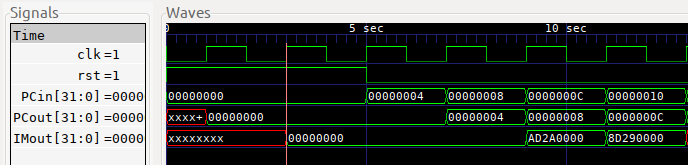
\includegraphics[width=\columnwidth]{Lab-Tex/Lab4-images/p2_1.png}
    \captionof{figure}{Wave output of program counter and instruction memory output}
    \medskip
\endgroup
\\

For this mini-program the \cc{ALUsrc} is set to \cc{1} so that the ALU accepts the sign-extended immediate value (which is the address offset) as its second argument. Because the offset in both the instructions is 0, we see that the \cc{ALUin2} is \cc{0x00000000} throughout.  \\

To have a more meaningful output, the \cc{\$t1} register was hard-coded to have \cc{0x00000001} as its value. This "address" with an offset of 0, results in the ALU output sum \cc{0x00000001}. So, the program will store to address \cc{0x00000001} in the data memory for the first instruction. It will load from that address as well for the second instruction.\\

\begingroup
    \centering
    \medskip
    %width=\columnwidth
    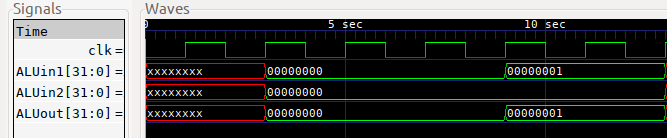
\includegraphics[width=\columnwidth]{Lab-Tex/Lab4-images/p2_2.png}
    \captionof{figure}{Wave output of the ALU}
    \medskip
\endgroup

Below are the inputs and outputs of the data memory. Since the first instruction is a \cc{sw} instruction, we see that the \cc{memWrite} signal is briefly enabled. The next instruction is the \cc{lw} instruction, hence the \cc{memRead} signal is enabled.\\

The \cc{address} signal refers to the data memory address. Before the first instruction is fetched, the address is default to \cc{0x00000000}. However, as is shown in the figure above, register \cc{\$t1} stores \cc{0x00000001}, which is used for both the instructions. \\
 
\begingroup
    \centering
    \medskip
    %width=\columnwidth
    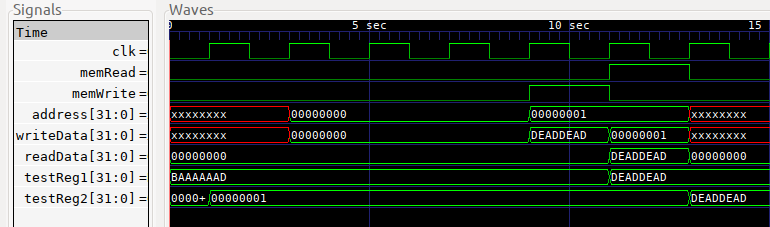
\includegraphics[width=\columnwidth]{Lab-Tex/Lab4-images/p2_3.png}
    \captionof{figure}{Wave output of the data memory and other relevant signals}
    \medskip
\endgroup

Note that in the figure above, \cc{testReg1} refers to the data memory address \cc{0x0000001}, while \cc{testReg2} refers to the register \cc{\&t1}. \\

Looking at the \cc{writeData} signal, we see that register \cc{\$t2} holds \cc{0xDEADDEAD}, which was stored into the data memory in the following clock cycle (see \cc{testReg1}). The original value of \cc{0xBAAAAAAD} was overwritten because of the \cc{sw} instruction. Also, it is worth noting that the data memory intakes \cc{0x00000001} as a \cc{writeData} value, but this has no effect because \cc{memWrite} signal is disabled by then. \\

The only change after \cc{sw} has been: 
\begin{lstlisting}
    dm.reg[1] = 0xBAAAAAAAD -> 0xDEADDEAD
\end{lstlisting}
\\

On the next cycle, which is a \cc{lw} instruction, the address in register \cc{\$t1} is offsetted by 0, resulting in  \cc{0x00000001}. So, the value in data memory at \cc{0x00000001} is written into register \cc{\$t1}. \\

Therefore, we see the \cc{readData} signal change from its default value of \cc{0x00000000} to \cc{0xDEADDEAD}, which is then reflected in the next clock cycle in register \cc{\$t1} (see \cc{testReg2}).\\

Thus, after \cc{lw}: 
\begin{lstlisting}
    $t1 = 0x00000001 -> 0xDEADDEAD
\end{lstlisting}
\\

This program demonstrates the CPU's ability to fetch from the instruction memory, read/write from a register, compute something in the ALU, and carry out store/load in the data memory. 


\section{Conclusion}

As a result of connecting all components, several questions were raised about the clocking in the CPU. Certain components, such as the PC and IM, were able to implement the clock, as shown by the staggered output waves. However, other components, such as the ALU, could not be clocked as it would lead to accidentally overwriting the value of a different register. When initially attempting this lab, all components were clocked, leading to incorrect behavior. The clocking was then incrementally rolled back until the program function as desired. It is understood that if no components were clocked, this would be a single-cycle CPU.\\

Nevertheless, going about it this way helped explain the difference between \cc{always @(*)} and \cc{always @(posedge clk)} blocks in Verilog. The former block is sensitive to any changes on the RHS of the "=" sign, and acts as the register version of the "assign" keyword. On the other hand, the \cc{always @(posedge clk)} block only updates the value on the LHS at the positive edge of the clock. \\

Working on this lab also clarified the difference between the "=" and "<=" operators. The former acts as a sequential assignments, where each value is assigned one after the other. On the other hand, the second operator allows for parallel assignment. \\

%%%%%%%%%%%%%%%%%%%%%%%%%%5
% BIBLIOGRAFIA 
% Estilo de bibliografia ABNT. Se não tiver instalado, mude para plain ou ieeetr

%\bibliographystyle{plain} % Inclua isso se não tiver ABNTEX instalado
% \begin{thebibliography}{refs}
% \bibitem{}
\printbibliography
% \end{thebibliography}
\end{document}